\documentclass[11pt]{article}
\usepackage[letterpaper]{geometry}
\usepackage{times}
\usepackage{verbatim}
\usepackage{graphicx}
\usepackage{float}
\usepackage{fullwidth}
\usepackage{amsmath}
\usepackage{amssymb}
\usepackage{fourier}
\usepackage{hyperref}
\graphicspath{{Images/}}
\title{ENGR-241 Transfer Function Lab}
\author{Jeremy Munson, Lauren Speirs \& Andrew Henrikson}
\geometry{top=.8in, bottom=.8in, left=.8in, right=.8in}

\setlength{\parindent}{0em}
\setlength{\parskip}{.5em}
\begin{document}
	\maketitle
	\subsection*{Overview}
	For this lab we calculated the transfer function then built the required circuit from the lab guidelines. We then calculated the voltage across the capacitor and compared our results from our circuits output to the oscilloscope. We then built the circuit using Orcad and analyzed the ciruit using the Laplace function in Pspice and compared its output to our previous results.
		\subsection*{Circuit Diagrams}
		\begin{figure}[H]
			\centering
			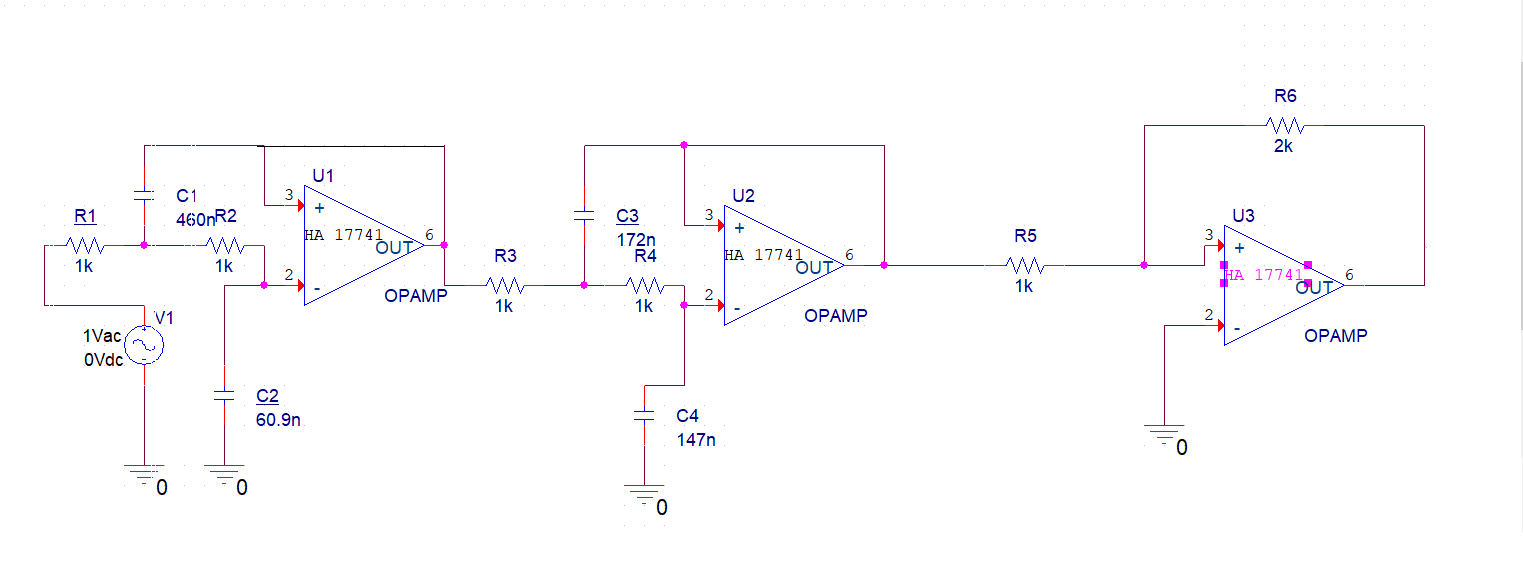
\includegraphics[width=5in]{images/diagram.png}
		\end{figure}
		
		Our suggested values and measured values for our components used are shown in the table below. The percent error is also listed.
		\begin{table}[H]
		\def\arraystretch{1.2}%
		\centering
		\begin{tabular}{|l|l|l|l|}
			
			\hline
			Components       	& Suggested 		& Measured      	&\% Diff	\\ \hline
			Resistor 1   		& $1 k\Omega$		& $0.998 k\Omega$   & -.2\%	     \\ \hline	
			Resistor 2			& $240 \Omega$		& $241 \Omega$      & 0.4\%       \\ \hline
			Inductor			& $220\mu H$		& $199\mu H$		& -10.6\%		\\ \hline
			Capacitor			& $1 \mu F$			& $0.95 \mu F$		& -5.3\%		\\ \hline
		\end{tabular}
	\end{table}

	
	\subsection*{Calculations}
	
	\subsubsection*{Finding $H(s)$}
	The circuit may be solved for $V(s)$ by using a simple voltage divider in the s domain.\\ 
	Find the equivalent impedance $Z_1= (240 \Omega + s \cdot L) \parallel \frac{1}{s\cdot c} = (s\cdot c+(240 \Omega + s \cdot L)^{-1})^{-1}$ \\
	Which makes $Z_{total}=Z_1+1k\Omega$ and the voltage divider equation yields $V_a=V_s\cdot \frac{Z_1}{Z_{total}}$\\
	Solving for $H(s)=\frac{V_a}{V_s}=\frac{Z_1}{Z_{total}}$ gives us\\
	$ H(s)= \left[\frac{1,000,000(11s+12,000,000)}{11s^2+12,000,000s+50,000,000,000}\right] \div \left[ \frac{1,000,000(11s+12,000,000)}{11s^2+12,000,000s+50,000,000,000}+1000\right]$\\
	Which simplifies to:
	\[ H(s)= \frac{1000(11s+12,000,000)}{11s^2+12,011,000s+62,000,000,000} \]
	\subsubsection*{Finding $V_a(s)$}
	We may simply multiply the transfer function by $V_s$\footnote{The input function, 5u(t) transforms to 5/s} to find $V_a$\\
	\[ H(s) \cdot \frac{5}{s}= \frac{5000(11s+12,000,000)}{11s^3+12,011,000s^2+62,000,000,000s} \]
	\newpage
	\subsubsection*{Finding $v_a(t)$}
	In order to find the time-domain expression for $v_a$ we must do an inverse laplace transform of $V_a(s)$. The function $V_a(s)$ is not transformable in it's current form, so we will expand it with partial fractions.
	\begin{itemize}
		\item The fraction is proper
		\item The denominator factors to $\frac{1}{11}\cdot s(11s-500\cdot (\sqrt{141,536,121}-12011))\cdot (11s+500(\sqrt{141,536,121}+12011))$
		\item Since there are 3 distinct real roots, we will have 3 constants to find. $K_1,K_2,K_3$
		\item Pull the $\frac{1}{11}$ up to the numerator, to simplify the expansion to follow.
		\item \[ \frac{55000(11s+12,000,000)}{s(11s-500\cdot (\sqrt{141,536,121}-12011))\cdot (11s+500(\sqrt{141,536,121}+12011))} =\] \\ \[ \frac{K_1}{s} + \frac{K_2}{(11s-500\cdot (\sqrt{141,536,121}-12,011))} \frac{K_3}{(11s+500(\sqrt{141,536,121}+12,011))}\]
		
		\item Multiplying by $s$, then evaluating at $s=0$ yields \[K_1=\frac{(55,000)(12,000,000)}{-500\cdot (\sqrt{141,536,121}-12,011)\cdot 500(\sqrt{141,536,121}+12,011)} = \frac{30}{31}\]
		
		\item Multiplying by $(11s-500\cdot (\sqrt{141536121}-12011))s$, then evaluating at $s=\frac{500}{11}\cdot (\sqrt{141536121}-12011) $ yields \[K_2 = \frac{-23353459965-1963060 \sqrt{141536121}}{4387619751} = -11\cdot\frac{30}{31} \]
		
		\item Multiplying by $(11s+500\cdot (\sqrt{141536121}+12011))$, then evaluating at $s=-\frac{500}{11}\cdot (\sqrt{141536121}+12011)$ yields \[K_3 = \frac{1963060 \sqrt{141536121}-23353459965}{4387619751} = \frac{3}{15313}\]
		
		\item The $K_1$ term inverse transforms to $\frac{30}{31}u(t)$
		\item The $K_2$ term inverse transforms to $-\frac{30}{31}\cdot e^{-\frac{500}{11}\cdot (12011-\sqrt{141536121})\cdot t}$
		\item The $K_3$ term inverse transforms to $\frac{3}{15313}\cdot e^{-\frac{500}{11}\cdot (12011+\sqrt{141536121})\cdot t}$
		
		\item The $K_3$ term is so small that it may reasonably be omitted here. \footnote{The error is $~196\mu v$ at $t=0$, and $~2\mu v$ by $4\mu s$}
		\item Evaluating the $K_2$ term numerically results in $-\frac{30}{31}e^{-5186.57\cdot t}$
		\item Finally, \[ v(t) = \frac{30}{31}\cdot(1-e^{-5186.57\cdot t})\cdot u(t) \]
	\end{itemize}
	
	\begin{figure}[H]
		\centering
		Plot of $v_a(t)$\\
		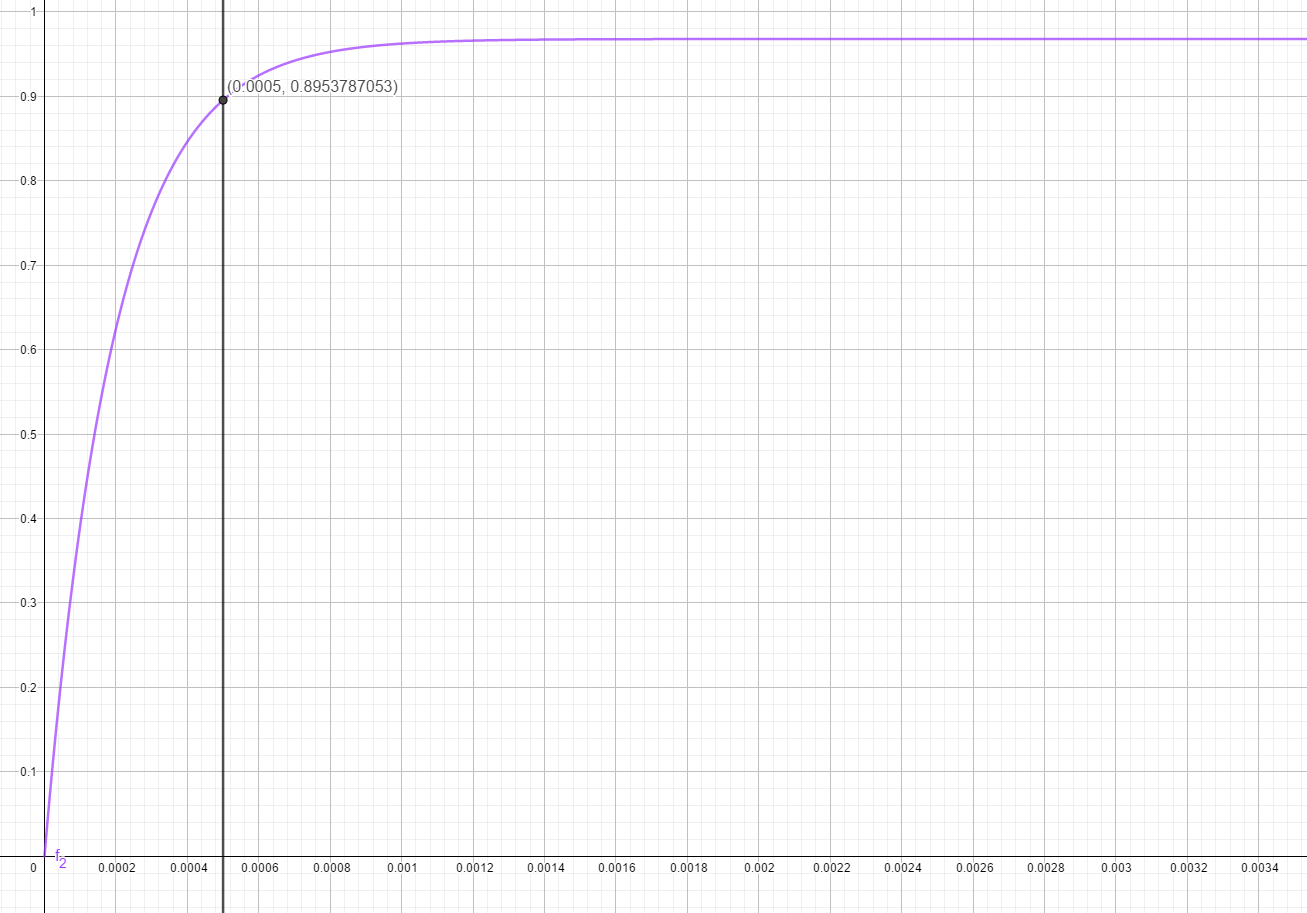
\includegraphics[width=6.55in]{images/function_graph.png}
	\end{figure}
	
	\subsection*{Procedure}
	The circuit was simple to construct using the breadboard. Aside from constructing the circuit as normal, we used the LCR meter to select a capacitor and an inductor that were as close to the exact values specified as possible. After constructing the circuit, measurements were taken in the usual manner using the oscilloscope. The circuits output is shown below.
		\begin{figure}[H]
		\centering
		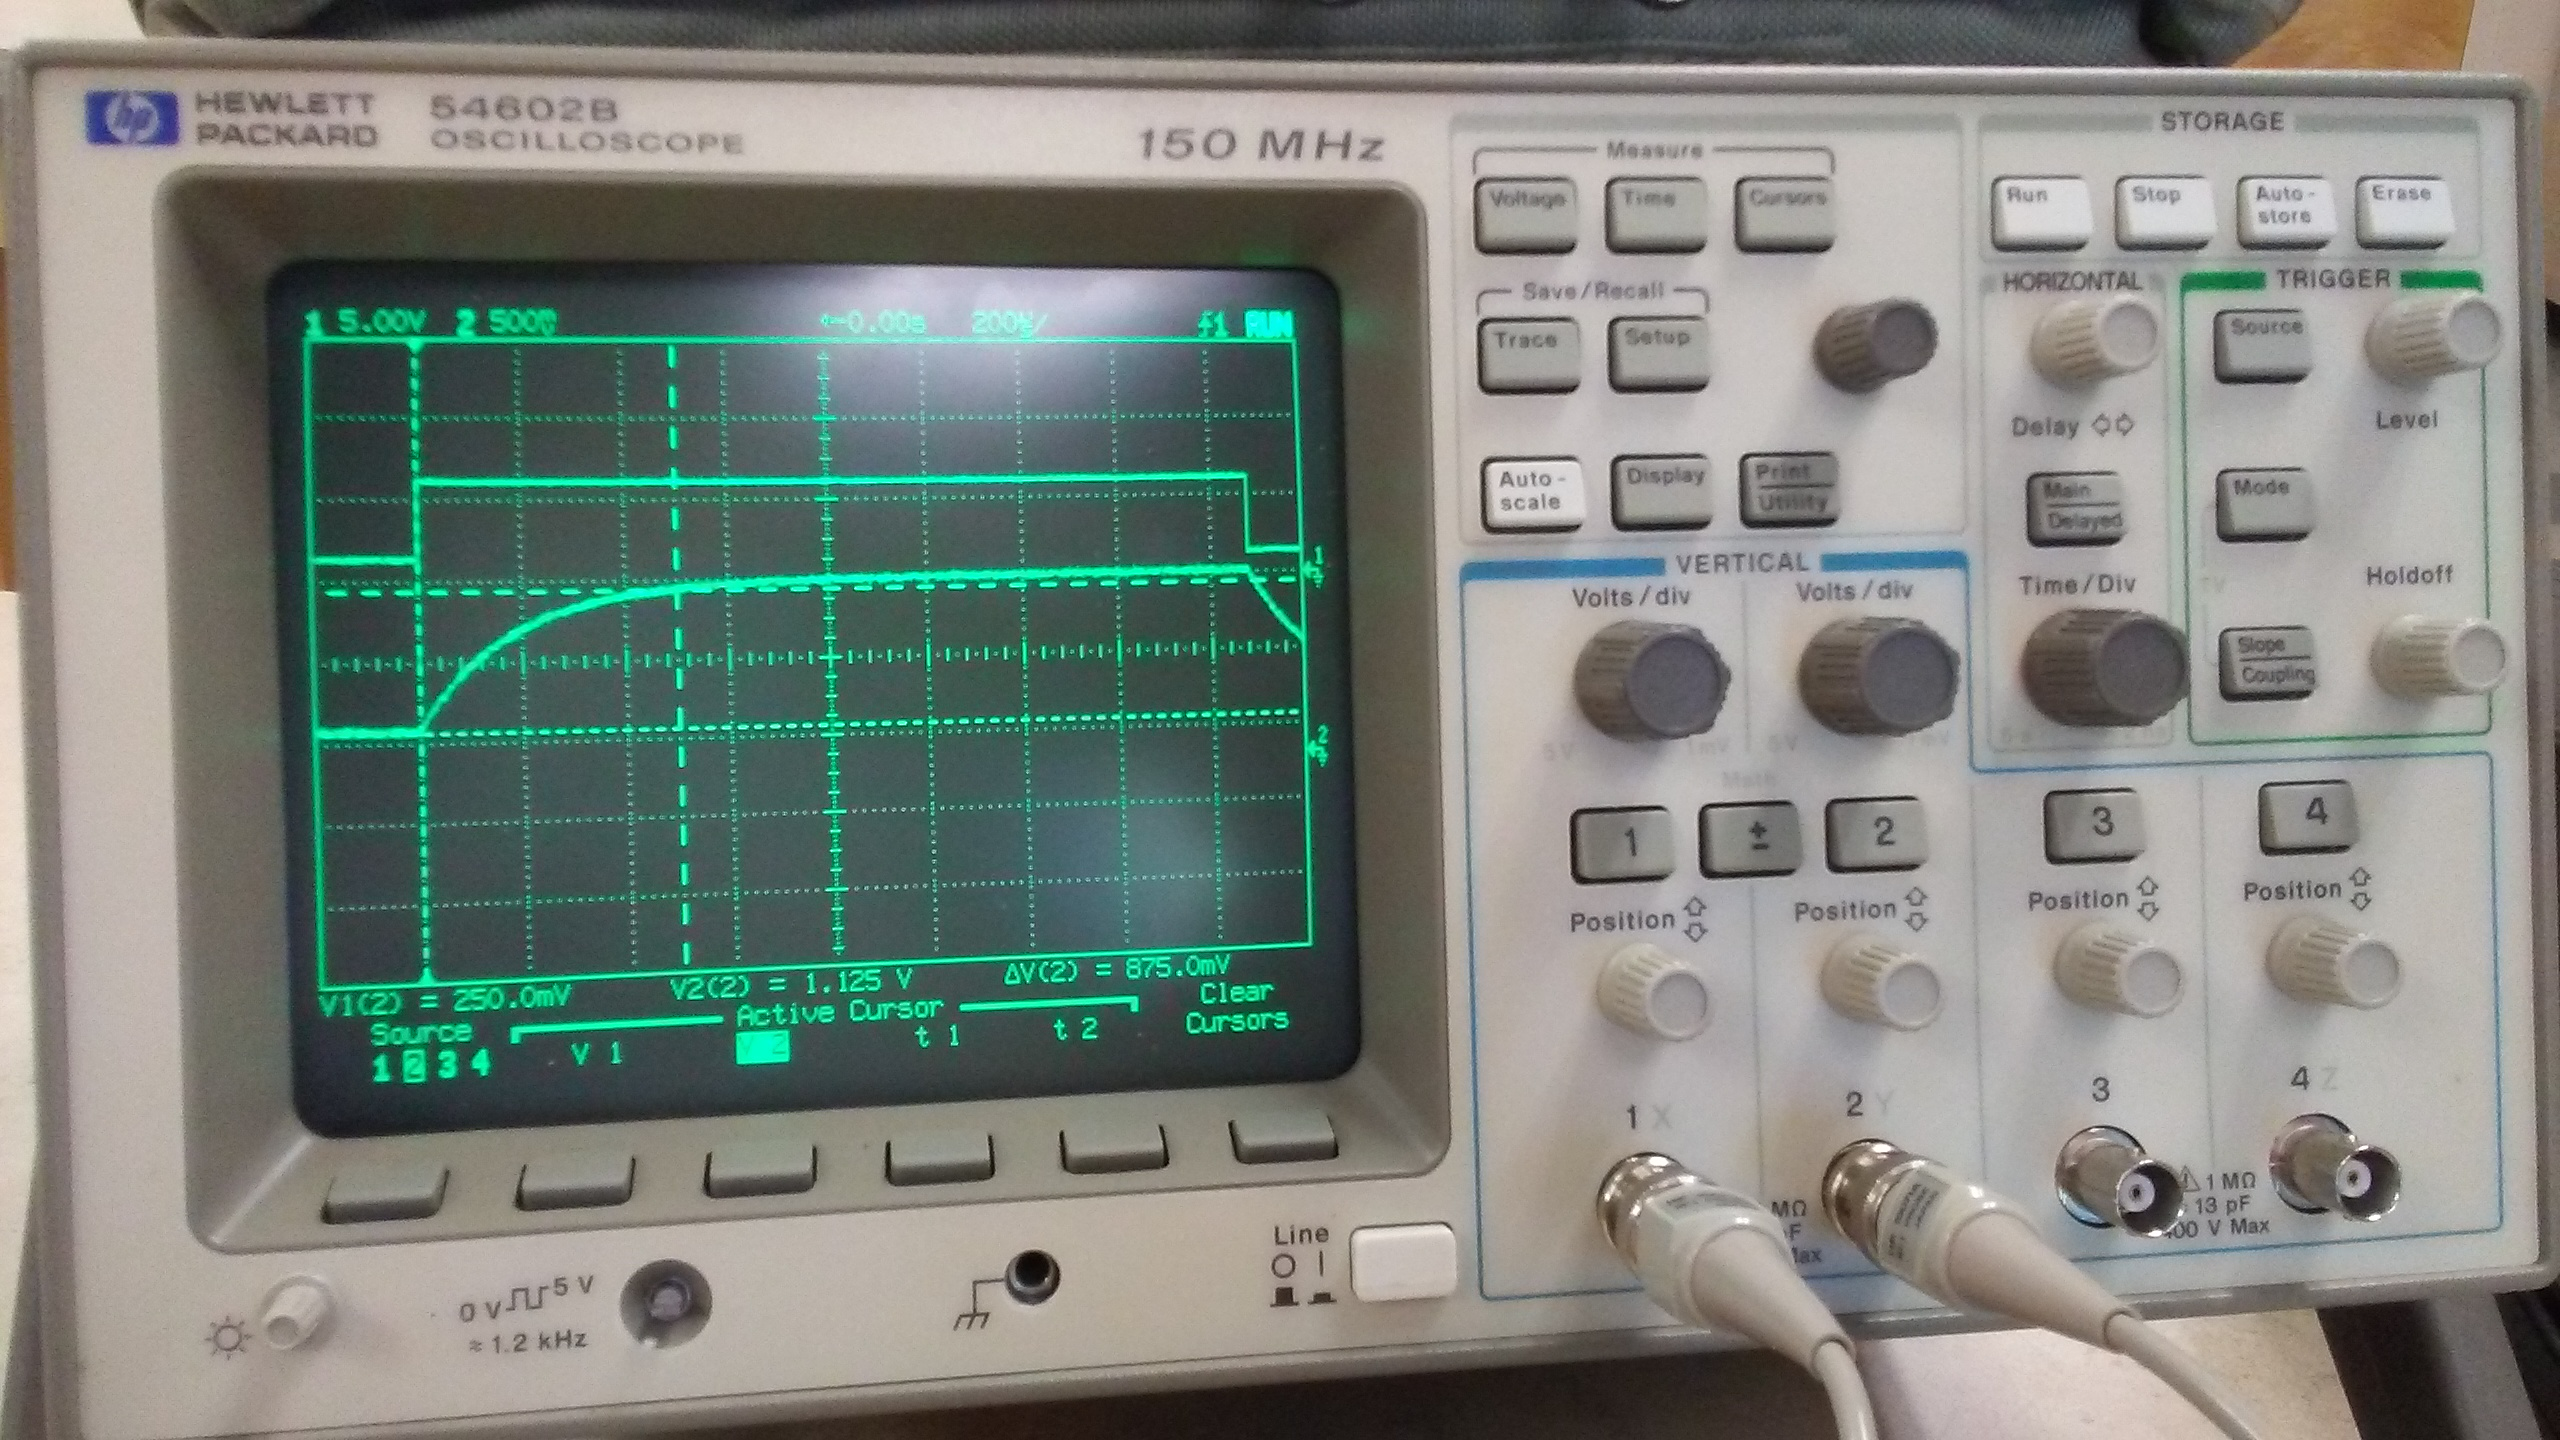
\includegraphics[width=5in]{images/oscilloscope_transfer.jpg}
		\end{figure}
	We then performed simulations of the same circuit in Orcad. The graph below is the output from the simulation.
		\begin{figure}[H]
		\centering
		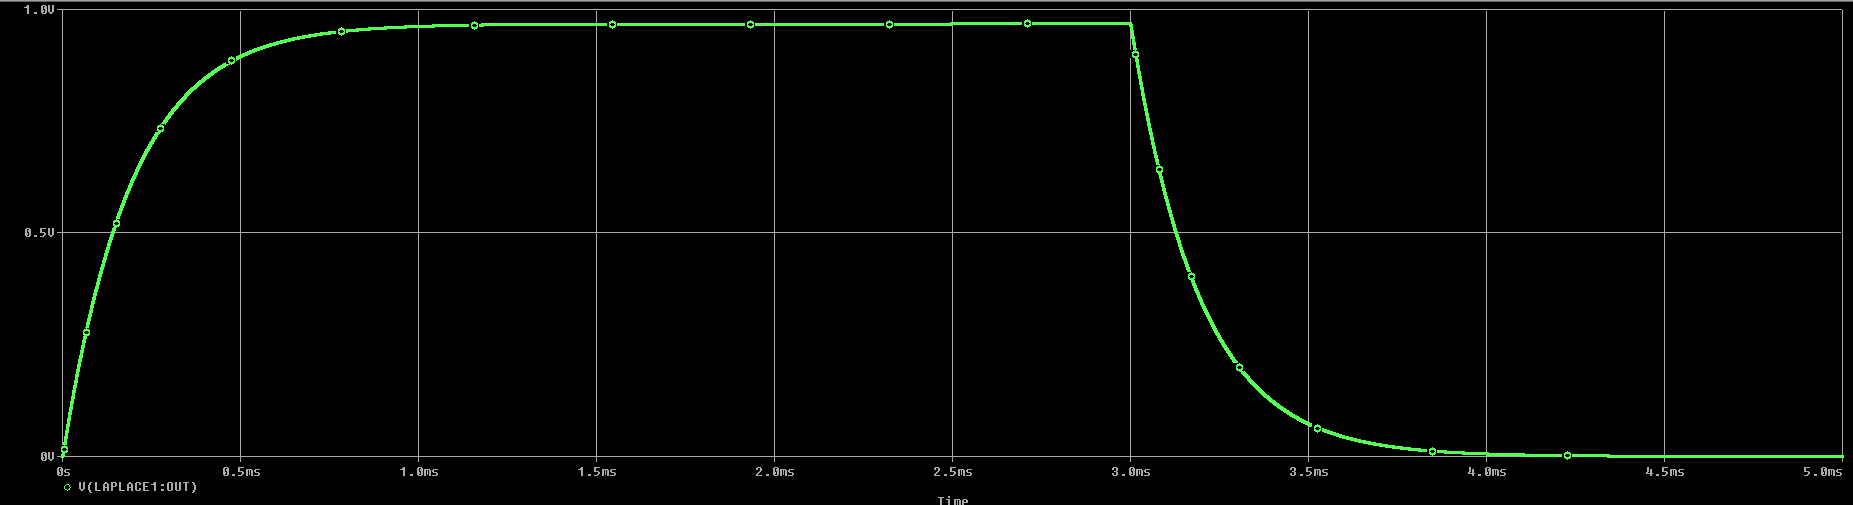
\includegraphics[width=6in]{images/simulated_curve.png}
		\end{figure}

	We subsequently used the Laplace feature in Orcad to verify our calculations. 
	
		\begin{figure}[H]
		\centering
		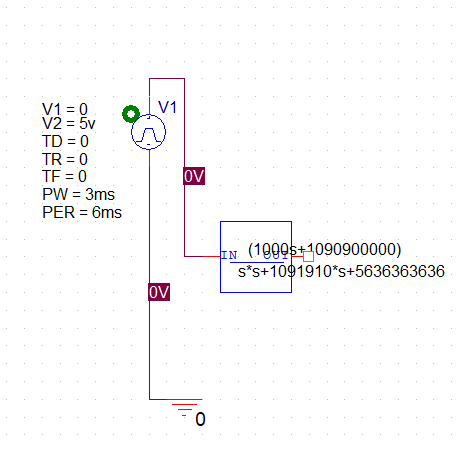
\includegraphics[width=5in]{images/simulation_schematic.png}
		\end{figure}
		\begin{figure}[H]
		\centering
		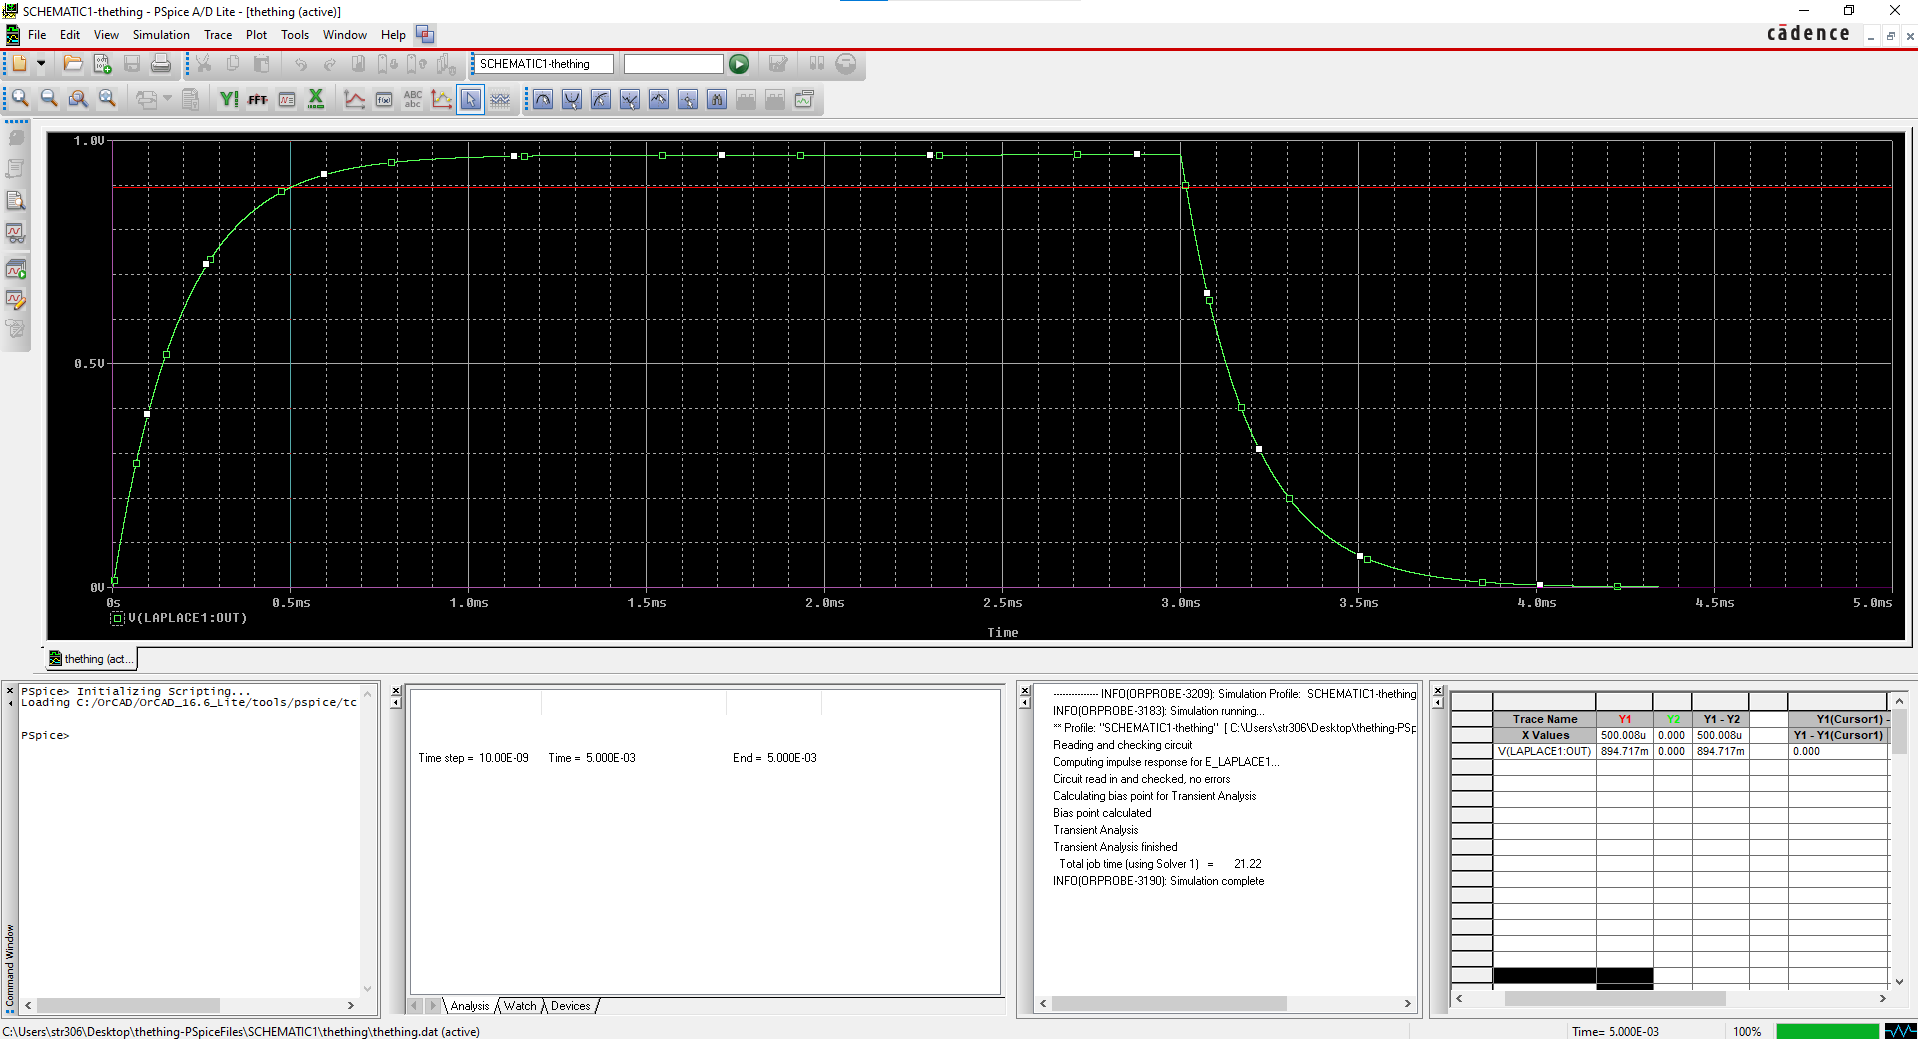
\includegraphics[width=5in]{images/laplace_part.png}
		\end{figure}
	

	\subsection*{Error Analysis}
	Error in this lab was extremely low. The largest error coming from the circuit we built due to not its components not being ideal. Also setting the frequency exactly at the required value is very difficult due to the touchy nature of the signal generator's controls. We were able to minimize the error from the components by measuring their real values on the LCR meter. All three functions approach approximately the same value at about 0.96V. The real circuit had slightly lower values than the simulated circuits.
	\subsection*{Conclusion}
	The lab was performed without issue. We were able to successfully calculate, simulate and build the circuit. Our results were excellent with minimal error. 
	
	
\end{document}
